% !TEX root = ../CedricDe Schepper2023_Thesis.tex

\section{Background}\label{sec:background}

% In a Background section, we describe the main concepts and/or techniques that are important for a reader to better understand the experiments. Usually, we divide the background into several subsections, one for each concept/technique.

% Figure~\ref{fig:ua-logo} is just an example of how to use the figure command.
% \begin{figure}[h]
% 	\centering
% 	
\includegraphics[width=0.3\textwidth]{images/ua.jpg} 
% 	\caption{University of Antwerp - Logo}
% 	\label{fig:ua-logo}
% \end{figure}

\subsection{Tabu Search}

Tabu Search is a metaheuristic search algorithm based on local search, a heuristic optimisation method that traverses the possible search space by performing local changes to the current solution. Since local search will only accept improving solutions, this traversal can end up being stuck in a local optimum. Tabu search is different from local search by relaxing this rule and also accepting worsening solutions. Additionally, tabu search maintains a memory structure to avoid changes being reversed. The usage of short- to long-term memory is  based on the assumption that optimisation techniques must incorporate memory to qualify as intelligent and that a bad strategic choice is superior to a good random choice\cite{glover1999}. This memory structure is implemented by maintaining a tabu list which contains the x most recent changes performed. A change is thus considered 'tabu' if it is present within the tabu list.
\\\\
Tabu search starts by constructing an initial solution. The solution can be generated randomly or by applying a deterministic approach. During the entire process, the best seen solution to date is maintained. This is necessary due to tabu search allowing worsening changes or so called moves to avoid getting trapped in local minima. After the solution initialisation, the iterative procedure starts searching for a feasible solution. This loop ends when  a specified stopping condition is met. This condition is generally a combination of a solution its objective function scoring below a certain threshold or the procedure reaching a maximum number of iterations.
\\\\
The first step of the main loop is to generate the complete list of possible neighbours of the current solution and ranking them based on the objective function. Subsequently, the best neighbour that is either not tabu or that meets the aspiration criterion is chosen as the next solution. A neighbour. A neighbour is considered tabu if it is present within the tabu list. The aspiration criterion is added to be able to override the tabu requirement. A possible aspiration is to accept solutions that are better than the best seen solution. After choosing the next solution, the best seen solution is updated if the newly generated solution is superior based on the objective function.
\\\\
When the stopping criteria is met, the algorithm ends and the best solution is returned. The full flow of the algorithm can be seen in Fig.\ref{fig:tabu-chart}.

\begin{figure}[h]
	\centering
	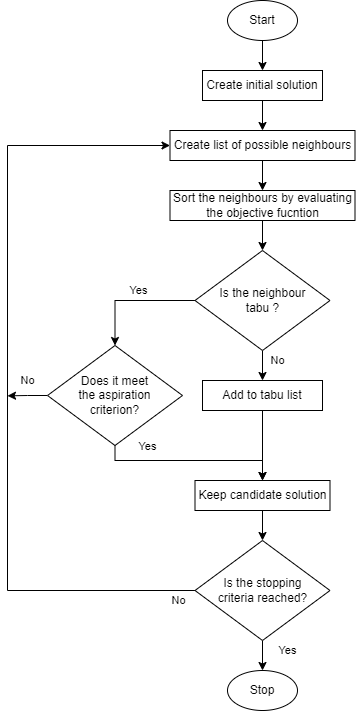
\includegraphics[width=0.5\textwidth]{images/tabu.drawio.png} 
	\caption{Tabu search flow}
	\label{fig:tabu-chart}
\end{figure}


 


